\section{Introduction}
\label{sec:intro}

We want to derive the kinematics of the $7$-degree-of-freedom robotic 
manipulator, minibot-7R. A kinematic diagram of the robot is provided 
in Figure~\ref{fig:minibot}.

\begin{figure}[h]
  \centering
  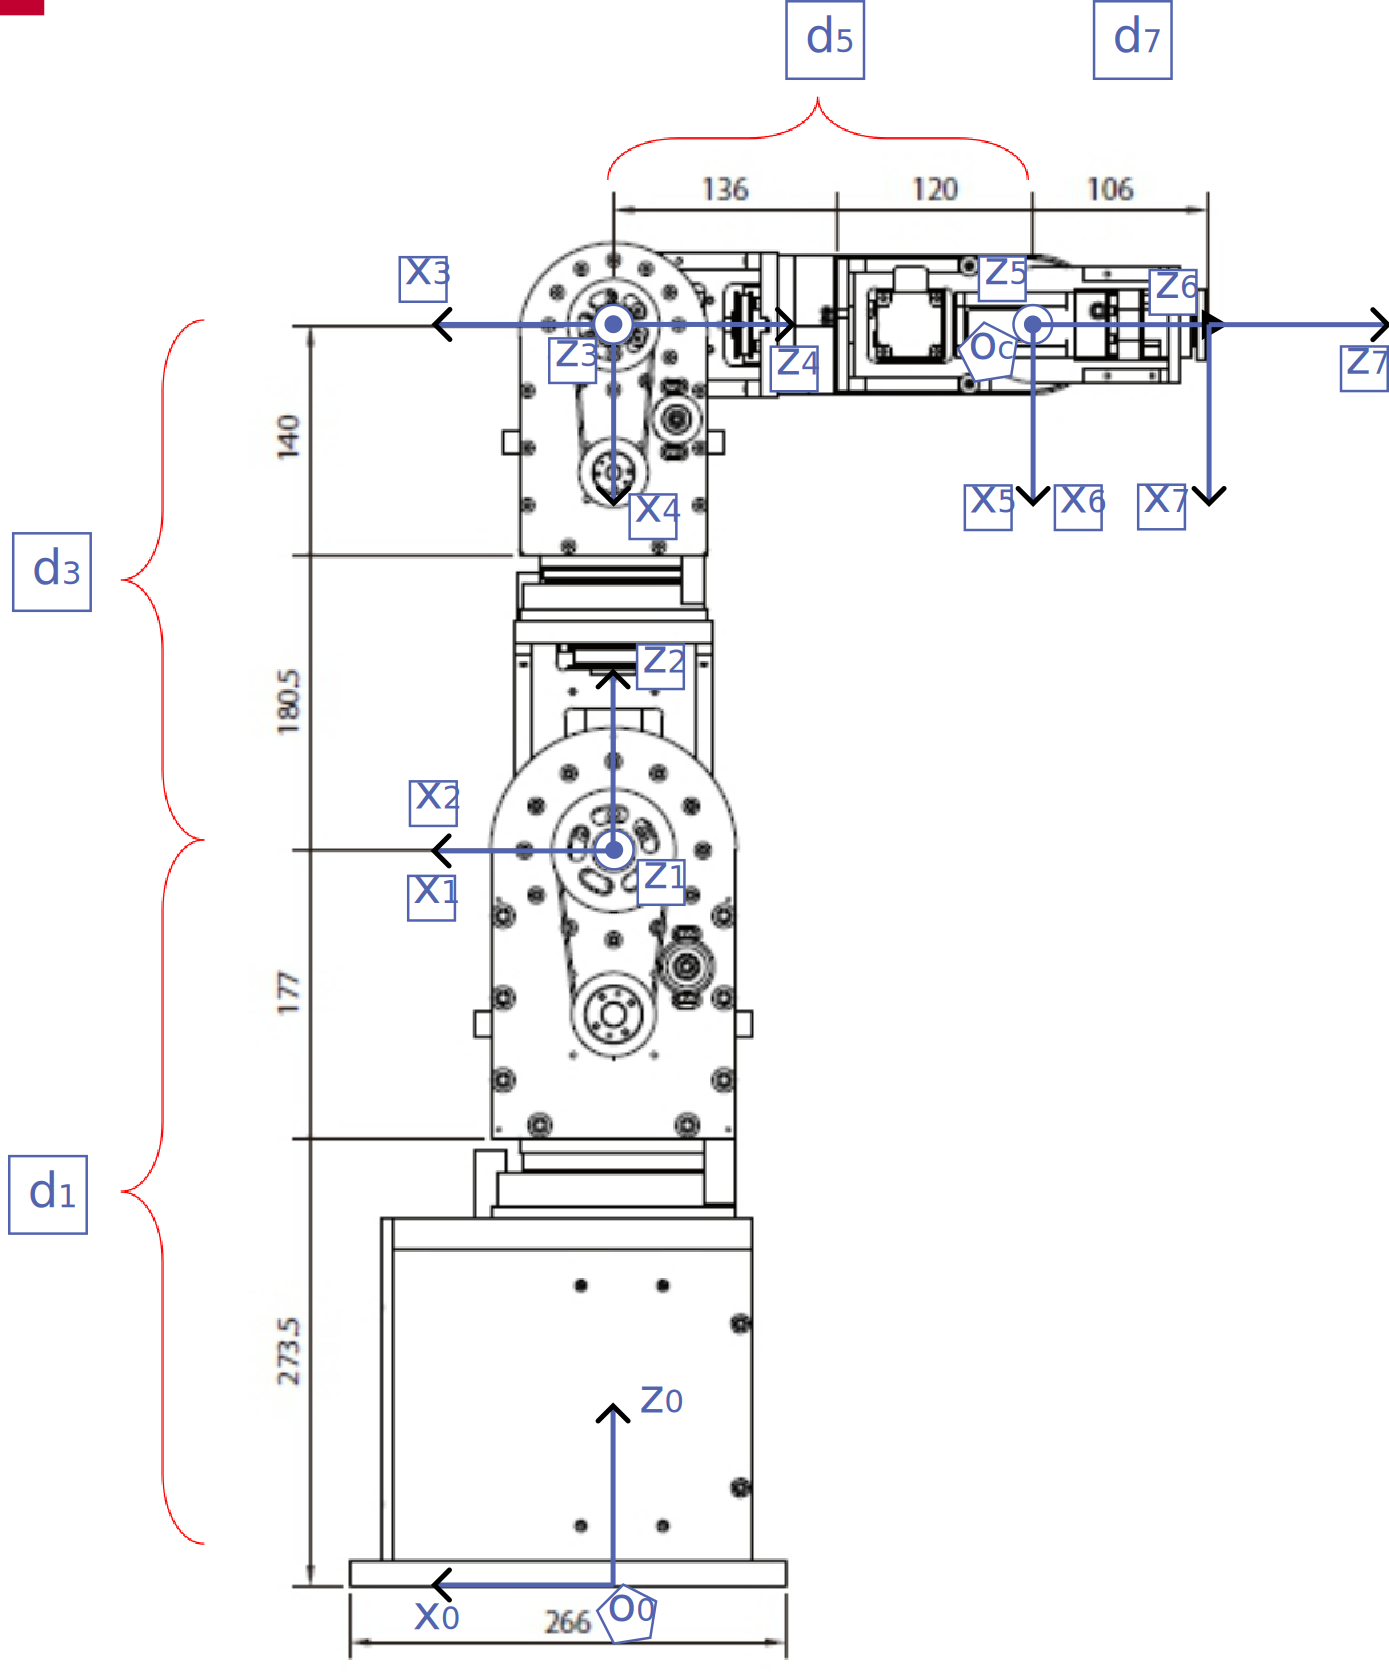
\includegraphics[width=0.5\textwidth]{./figures/minibot-7R.eps}
  \caption{Schematic of minibot-7R.}
  \label{fig:minibot}
\end{figure}

We will follow the classic Denavit-Hartenberg convention as presented 
in~\cite{spong2020robot}.
